\documentclass[a4paper, parskip=half]{scrartcl}

%{{{ Packages

\usepackage{fontspec}
\usepackage{tikz}
\usepackage[scale=2]{ccicons}

%}}}
% {{{ Fonts

\setmainfont{Linux Libertine O}
\setsansfont[BoldFont={* Semibold}]{Source Sans Pro}

% }}}
%{{{ TikZ

\usetikzlibrary{calc}

\tikzset{
  string/.style={
    line width={1.5pt},
    color=black!60,
  },
  fret/.style={
    line width={1pt},
    color=black!30,
  },
  fretted/.style={
    fill=white,
    draw=black!90,
    circle,
    inner sep=2.5pt,
  },
}

\newcommand{\addfingering}[2][10]{%
  \def\data{#2}
  \def\nfrets{#1}
  \pgfmathsetmacro\nfretsm{1+\nfrets}
  % frets
  \foreach \x in {1, ..., \nfrets}
    \draw[fret] (\x, 0) -- (\x, 1.95);

  % strings
  \foreach \y in {0, 0.65, 1.3, 1.95}
    \draw[string] (0, \y) -- (\nfretsm, \y);

  \foreach \x / \y / \z [count=\ni]  in \data{%
    \pgfmathsetmacro\yr{0.65*\y}
    \node[fretted] (fretted-\ni) at (\x, \yr) {\z};
  }
}

% }}}
% {{{ Meta

\title{\vspace{-3em}Electric Bass Patterns}
\author{Matthias Vogelgesang}
\date{}

%}}}

\begin{document}
\maketitle

\section{Introduction}

This short document lists finger patterns covering arpeggios and scales on a
four string electric bass guitar. Although they are written as purely technical
exercises, they should be practiced within a musical context. That means run
them up and down the neck to a tune from the Real Book or a chord drone.

\section{Arpeggios}

\subsection{First inversion}

All arpeggios start with the major or minor third up to the root.


\subsubsection*{Major 7th}

The first pattern is easily recognizable as a minor 6th arpeggio.
\vspace{1em}

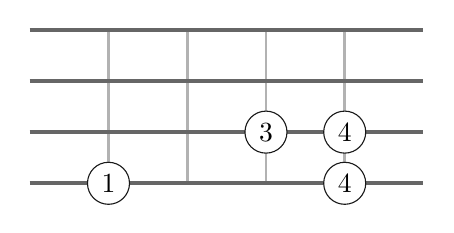
\begin{tikzpicture}
  \addfingering[4]{%
    1/0/1, 4/0/4,
    3/1/3, 4/1/4
  }
\end{tikzpicture}
\hspace{1em}
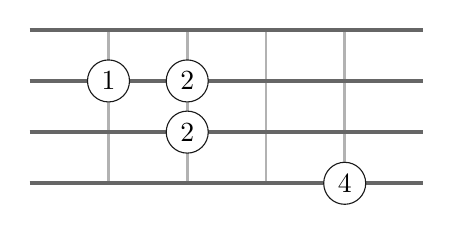
\begin{tikzpicture}
  \addfingering[4]{%
    4/0/4,
    2/1/2,
    1/2/1, 2/2/2
  }
\end{tikzpicture}


\subsubsection*{Dominant 7th}

The first inversion of a dominant 7th looks like a half-diminished triad with an
additional 6.

\vspace{1em}

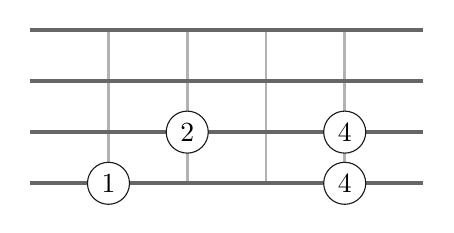
\begin{tikzpicture}
  \addfingering[4]{%
    1/0/1, 4/0/4,
    2/1/2, 4/1/4
  }
\end{tikzpicture}
\hspace{1em}
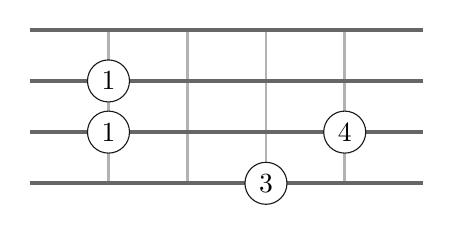
\begin{tikzpicture}
  \addfingering[4]{%
    3/0/3,
    1/1/1, 4/1/4,
    1/2/1
  }
\end{tikzpicture}


\subsubsection*{Minor 7th}

Just like the inversion of a major 7th forms a minor 6th, the first inversion of
a minor 7th is a major 6th.
\vspace{1em}

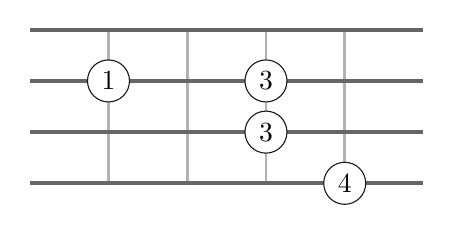
\begin{tikzpicture}
  \addfingering[4]{%
    4/0/4,
    3/1/3,
    1/2/1, 3/2/3
  }
\end{tikzpicture}
\hspace{1em}
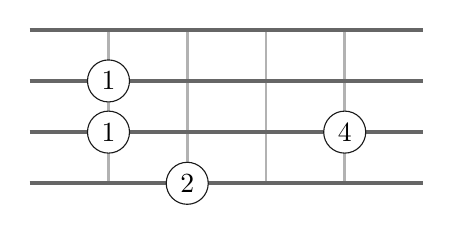
\begin{tikzpicture}
  \addfingering[4]{%
    2/0/2,
    1/1/1, 4/1/4,
    1/2/1
  }
\end{tikzpicture}


\subsubsection*{Half-dimished 7th}

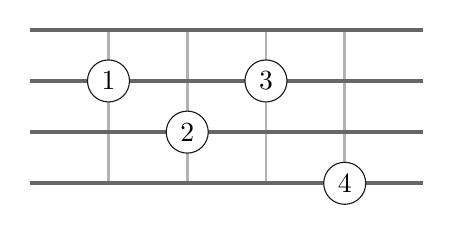
\begin{tikzpicture}
  \addfingering[4]{%
    4/0/4,
    2/1/2,
    1/2/1, 3/2/3
  }
\end{tikzpicture}


\section{Scales}

\subsection{Major}

One-octave major scale starting with \emph{second} and \emph{first} finger.
\vspace{1em}

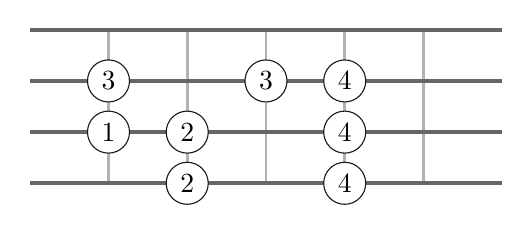
\begin{tikzpicture}
  \addfingering[5]{%
    2/0/2, 4/0/4,
    1/1/1, 2/1/2, 4/1/4,
    1/2/3, 3/2/3, 4/2/4
  }
\end{tikzpicture}
\hspace{1em}
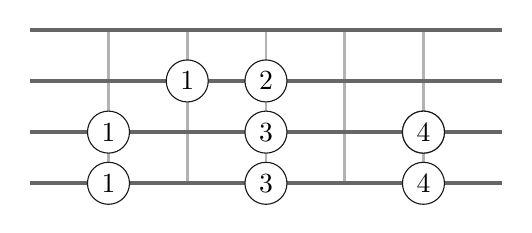
\begin{tikzpicture}
  \addfingering[5]{%
    1/0/1, 3/0/3, 5/0/4,
    1/1/1, 3/1/3, 5/1/4,
    2/2/1, 3/2/2, 5/1/4
  }
\end{tikzpicture}\\

Two-octave major scale starting on the E-string.
\vspace{1em}

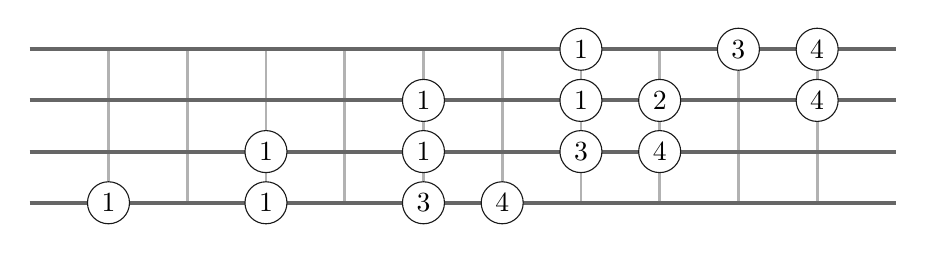
\begin{tikzpicture}
  \addfingering[10]{%
    1/0/1, 3/0/1, 5/0/3, 6/0/4,
    3/1/1, 5/1/1, 7/1/3, 8/1/4,
    5/2/1, 7/2/1, 8/2/2, 10/2/4,
    7/3/1, 9/3/3, 10/3/4
  }
\end{tikzpicture}


\subsection{Dorian}

One-octave dorian starting on E-string.

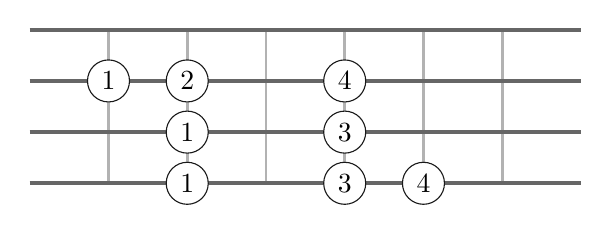
\begin{tikzpicture}
  \addfingering[6]{%
    2/0/1, 4/0/3, 5/0/4,
    2/1/1, 4/1/3,
    1/2/1, 2/2/2, 4/2/4
  }
\end{tikzpicture}

Two-octave dorian starting on E-string.

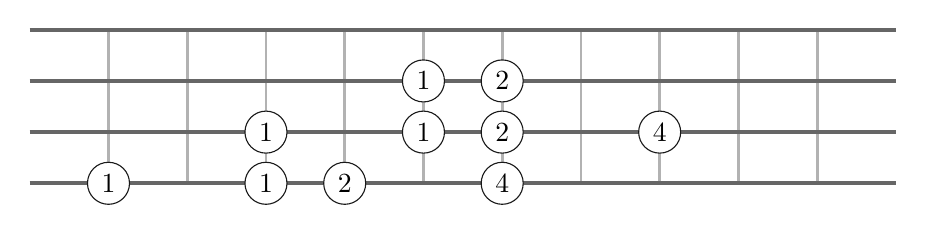
\begin{tikzpicture}
  \addfingering[10]{%
    1/0/1, 3/0/1, 4/0/2, 6/0/4,
    3/1/1, 5/1/1, 6/1/2, 8/1/4,
    5/2/1, 6/2/2
  }
\end{tikzpicture}

\subsection{Melodic minor}

One-octave melodic minor. Similar to Dorian mode but with a major 7th instead.

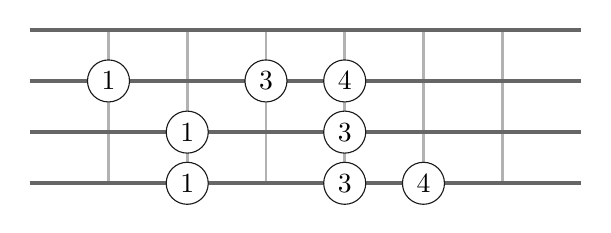
\begin{tikzpicture}
  \addfingering[6]{%
    2/0/1, 4/0/3, 5/0/4,
    2/1/1, 4/1/3,
    1/2/1, 3/2/3, 4/2/4
  }
\end{tikzpicture}


\subsection{Harmonic minor}

One-octave harmonic minor scale. Unfortunately, the step from seventh to octave
prevents any nicer fingerings.
\vspace{1em}

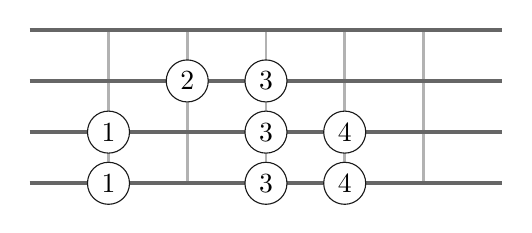
\begin{tikzpicture}
  \addfingering[5]{%
    1/0/1, 3/0/3, 4/0/4,
    1/1/1, 3/1/3, 4/1/4,
    2/2/2, 3/2/3
  }
\end{tikzpicture}


\section{Additional information}

This work is licensed under \emph{Creative Commons Attribution-ShareAlike 4.0
International}.

\begin{center}\ccbysa\end{center}

\end{document}
